\documentclass[a4paper,fleqn,twoside,12pt]{article}

%%%%%%%%%%%%%%%%%%%%


\usepackage[]{geometry}
\usepackage[latin1, utf8]{inputenc}
\usepackage[UKenglish]{babel}
\usepackage[UKenglish]{isodate}
\usepackage{amsmath}
\usepackage{amsfonts}
\usepackage{amssymb}
\usepackage{amsthm}
\usepackage{graphicx}
\usepackage{chngpage}
\usepackage{calc}
\PassOptionsToPackage{hyphens}{url}
\usepackage{hyperref}
\usepackage[nameinlink]{cleveref}
\usepackage{fancyhdr}
\usepackage{titletoc}
\usepackage[explicit]{titlesec}
\usepackage[square,numbers]{natbib}
\usepackage[dvipsnames]{xcolor}
\usepackage[sc]{mathpazo}
\linespread{1.05}
\usepackage[T1]{fontenc}
\usepackage{minted}
\usepackage[export]{adjustbox}

\hypersetup{
	colorlinks=true,
	linkcolor=black,
	urlcolor=black,
	citecolor=black
}

\setlength{\parindent}{0mm}
\setlength{\parskip}{\medskipamount}
\renewcommand\baselinestretch{1.2}

\cleanlookdateon

\makeatletter
\newcommand{\@assignment}[0]{Assignment}
\newcommand{\assignment}[1]{\renewcommand{\@assignment}{#1}}
\newcommand{\@supervisor}[0]{}
\newcommand{\supervisor}[1]{\renewcommand{\@supervisor}{#1}}
\newcommand{\@yearofstudy}[0]{}
\newcommand{\yearofstudy}[1]{\renewcommand{\@yearofstudy}{#1}}
\makeatletter

\newtoggle{IsDissertation}

%%%%%%%%%%%%%%%%%%%%%%%%%%%%%%%%%%%%%%%%%%%%%%%%%%%%%%%%%%%%%%%%%%%%%%%%%%%%%%%
%% Project-specific configuration
%%%%%%%%%%%%%%%%%%%%%%%%%%%%%%%%%%%%%%%%%%%%%%%%%%%%%%%%%%%%%%%%%%%%%%%%%%%%%%%

\author{Your name}
\title{Project title}
% \supervisor{Your supervisor's name}
% \yearofstudy{3\textsuperscript{rd}}

%%%%%%%%%%%%%%%%%%%%%%%%%%%%%%%%%%%%%%%%%%%%%%%%%%%%%%%%%%%%%%%%%%%%%%%%%%%%%%%


\assignment{Progress report}

%%%%%%%%%%%%%%%%%%%%

\pagestyle{plain}
\renewcommand{\headrulewidth}{0.0pt}

\makeatletter
\fancypagestyle{plain}{
	\fancyhf{}
	%\fancyhead[R]{\textit{\@title} - \textit{\@assignment}}
	%\fancyhead[L]{\textit{\@author}}
	\fancyfoot[C]{\thepage}
}
\makeatother

%%%%%%%%%%%%%%%%%%%%

\begin{document}

\makeatletter
\begin{titlepage}

    % do not show the assignment name for the dissertation
    \iftoggle{IsDissertation}
    {
        \textbf{\Huge \@title} \\[1.5cm]
    }
    {
        \textbf{\Huge \@title} \\
        \Large \@assignment \\[1.5cm]
    }
    \Large \textbf{\@author} \\
    Department of Computer Science \\
    University of Warwick \\

    % include the supervisor and year of study if the are specified and its the disseration
    \iftoggle{IsDissertation}{
        \ifdefempty{\@supervisor}{}{
            Supervised by \@supervisor \\
        }\ifdefempty{\@yearofstudy}{}{
            Year of Study: \@yearofstudy \\
        }
    }{}

    \vfill

    % include the current date for the dissertation
    \iftoggle{IsDissertation}{\today}{}

    \begin{adjustwidth}{-\oddsidemargin-1in}{-\rightmargin}
        \centering
        
\includegraphics[width=\paperwidth]{../common/line.png}
    \end{adjustwidth}

    \vspace*{-3.5cm}

\end{titlepage}
\makeatother


\pagestyle{plain}
\section{Introduction}
In recent years processors have been running into limits in single-threaded processing speed \cite{cpu_clk_speed}. Overall performance has been increased by taking advantage of parallelism. This can be achieved using multiple cores to gain general parallelism or through hardware accelerators specifically designed to exploit the parallelism inherent in an algorithm. An example would be multiplying matrices. Many matrix operations involve computing many simpler calculations on the components of the matrix. These calculations are often independent and can be performed in parallel. A processor would compute these sequentially but a specific hardware implementation would be able to compute them in parallel.

An FPGA allows hardware to be developed and iterated on much faster than other options such as using an ASIC or logic ICs. They allow hardware to be designed with HDL code that is then constructed on the FPGA \cite{whatisanfpga}. For this reason, they will be used in this project to implement the accelerator. Some FPGA boards have a built-in processor but the board used in this project does not so that will also be constructed on the FPGA.

RISC-V is a good option for this processor as it is an open standard instruction set architecture \cite{risc} that can be implemented by anyone and has multiple options for FPGA implementations such as Rocket Chip \cite{rocketchip}. It is also used extensively in other products such as high-performance SiFive boards and the low-power Espressif's ESP32-C3 microcontroller. Because of this adoption, more libraries are available such as a port of Debian.

\newpage
\subsection{Objectives}

Develop a hardware accelerator for a RISC-V processor communicating over the AXI bus and compare it against a bare-metal software solution.

\begin{itemize}
	\item Generate a RISC-V core on an FPGA and run bare-metal code on it (Must).
	\item Design an IP block that connects to the RISC-V's AXI bus that can send and receive data (Must).
	\item Design an IP block that performs the hardware-accelerated functionality (Must).
	\item Develop a driver in bare-metal C code to use the accelerator (Must).
	\item Design and implement a test for the accelerator (Must).
	\item Implement the test using a software approach and compare results (Should).
	\item Implement a hardware accelerator using an alternative method of communication such as an APB bus and compare (Could)
	\item Run Linux on the processor and make the accelerator available for use (Won't)
\end{itemize}

\newpage

\subsection{Related Work}
\subsubsection{Work A - Implementation of a RISC-V Processor with Hardware Accelerator \cite{risc-v_hard_accel}}
This paper covers the development of a hardware matrix multiplier for a RISC-V processer. They used a ZedBoard which uses the same Artix-7 FPGA chip as the Nexys A7 100T that this project uses. They use PULPino \cite{pulpino}, a 32-bit single-core RISC-V microprocessor. This project does not support the Nexys A7 100T FPGA used in our project so vivado-risk-v \cite{vivado-risk-v} is used to generate a 64-bit RISC-V core using the Rocket Chip project \cite{rocketchip}. This takes more of the resources available to the FPGA but can be reduced to 32-bit if needed as we will not be running Linux. They used the APB bus to communicate between the accelerator and PULPino microprocessor due to its interface being simpler than the AXI bus. In our project, the AXI interface will be used as it is recommended by the base project and provides the option for higher-performance transfers. When tested their accelerator reduced the number of clock cycles required from 603 to 134. This is a good improvement but due to the processor having a clock speed of 5 MHz, it is unable to compete with modern processors. They encountered many errors when trying to build C programs for the PULPino and required much trial and error. The process for compiling code for our project has proved much simpler.

\subsubsection{Work B - Matrix Multiplication Accelerator \citep{matrix_mult_accel}}
This paper also used an accelerator for matrix multiplication but with a DE1-SoC board using a built-in ARM Cortex-A9 HPS as the processer and a Cyclone V FPGA. They used parallel ports to communicate between the HPS and FPGA \cite{pio}. Two approaches were used based on the naive method. The first was to store the input matrices in two registers and use massive parallelization to set the values in the output register. This allowed values to be accessed with zero cycles of latency and in parallel but is very hard to scale. The other method used M10k memory blocks to store the inputs. These only have a single read port and write port limiting the ability to exploit parallelism so they opted to improve performance by pipelining and increasing clock speeds. Their tests showed that the HPS performed better than their accelerator but performed significantly more consistently than the HPS. The accelerator and HPS ran at very different clock speeds, 100MHz and 925MHz. As the tests measured runtime in ms this would have heavily benefited the HPS. A clock cycle test as used in "Implementation of a RISC-V Processor with Hardware Accelerator" may have provided more comparable results.

\subsubsection{Comparison}
\begin{table}[H]
	\centering
	\resizebox{\textwidth}{!}{%
		\begin{tabular}{c|c|c|}
			\cline{2-3}
			& \begin{tabular}[c]{@{}c@{}}Implementation of a RISC-V Processor\\ with Hardware Accelerator\end{tabular}                                      & Matrix Multiplication Accelerator                                                                                                                                                                                                    \\ \hline
			\multicolumn{1}{|c|}{\begin{tabular}[c]{@{}c@{}}Development Board\\ Used\end{tabular}} & \begin{tabular}[c]{@{}c@{}}ZedBoard - Artix-7 and \\ ARM Cortex-A9 MPcore\end{tabular}                                                        & \begin{tabular}[c]{@{}c@{}}DE1-SoC - Cyclone V and \\ ARM Cortex-A9\end{tabular}                                                                                                                                                     \\ \hline
			\multicolumn{1}{|c|}{Processor Used}                                                   & PULPino (RISC-V) on FPGA                                                                                                                      & ARM Cortex-A9 HPS                                                                                                                                                                                                                    \\ \hline
			\multicolumn{1}{|c|}{Communication Method}                                             & APB bus                                                                                                                                       & Parallel Port                                                                                                                                                                                                                        \\ \hline
			\multicolumn{1}{|c|}{Algorithm Used}                                                   & Naive method with parallelism                                                                                                                 & \begin{tabular}[c]{@{}c@{}}Naive method using massive parallelism and \\ "single-threaded" with heavy  pipelining\end{tabular}                                                                                                       \\ \hline
			\multicolumn{1}{|c|}{Testing}                                                          & \begin{tabular}[c]{@{}c@{}}Measures clock cycles required to complete\\  a 4x4 matrix multiplication in \\ hardware and software\end{tabular} & \begin{tabular}[c]{@{}c@{}}Measured runtime (ms) to compute 20x20, 40x40, \\ 60x60 and 80x80 matrix multiplications \\ in hardware and software\\ Measured power usage (W) for hardware and \\ software implementations\end{tabular} \\ \hline
		\end{tabular}%
	}
	\caption{Comparison Table of Related Works}
	\label{tab:comp}
\end{table}

Both works use development boards with a HPS but work A is using the PULPino microcontroller implemented on the FPGA instead. This is a lower-performance processor but allows a greater level of control over the design. They use the APB bus to attach their accelerator while work B uses a parallel port that is built into the chip to connect the HPS and FPGA.

Work A implements a 4x4 matrix accelerator exploiting parallelism. This method is not scalable in hardware due to the exponential increase in hardware required as the matrix size increases. Block matrix multiplication can be used to split larger matrices into a size that is compatible with the accelerator decreasing the impact of this issue. Work B also looked at this method but decided to use a more scalable design by creating a single module that calculates one value of the output matrix and makes heavy use of pipelining to make this process more efficient. This takes more steps to complete a calculation but can handle far bigger matrices. For this project, the method used will need to be evaluated for how important scalability is compared to performance.

Work B has tested their design with 4 different matrix sizes 20, 40, 60 and 80 while work A has used only the 4x4 matrix that is directly compatible with their accelerator. They have used different methods of testing, work A uses clock cycles to measure execution time. This allows for excellent comparisons between the hardware and software approaches as it removes the impact of any difference in clock rates. Work B uses runtime in ms which showed lower performance for their accelerator than software implementation. The HPS used runs with a clock speed 9.25x faster than the accelerator giving it an advantage in this test which may explain the results. Work B also tested power usage which showed the accelerator was more power efficient. For this project clock cycles seem to be a better method of performance testing but power usage also provides interesting data about how beneficial an accelerator could be.
\section{Background}
\label{sec:background}

\subsection{Base project: vivado-risc-v}
This project uses Rocket Chip to generate RISC-V processors that can be run on various FPGAs. It provides enough documentation to build a core and flash it to the board but very little else. There is some documentation on adding a peripheral device and making it available in Linux but I was unable to get this to work and further research into how to add to the device tree resulted in limited information. It provides an example bare-metal file that can be used as a base for new code but there was no documentation on it.

\subsection{AXI protocol}
The AXI4 protocol is used to communicate with custom IP blocks \cite{axi}. There are 3 interfaces AXI4, AXI4-Lite and AXI4-Stream. AXI4 provides high-performance memory-mapped communication and AXI4-Stream allows for high-speed streaming of data. For this project, AXI4-Lite will be used as it is a simpler interface for low-throughput memory-mapped communication. This will limit the performance of the accelerator but will simplify development. The project will be designed in a modular way to allow the interface block to be changed without needing to modify the accelertor allowing the option to utilise the higher-performance AXI4 interface in the future.

\subsection{Hardware Acceleration}
A hardware accelerator is a block of hardware designed to fully exploit the parallelism available in an algorithm. An example would be matrix multiplication. The naive method takes $\mathcal{O}(n^{3})$ time which can be optimised by more complicated algorithms to $\mathcal{O}(n^{2.3728596})$ \citep{alman2020refined}. Looking at the naive algorithm, it shows that while many operations are needed all the multiplications can be done in parallel and then added to generate the result. A hardware device would be able to do this allowing for it to be completed in constant time but would face issues with scaling.

Another possible application is in image processing with local filters \cite{image_process}. A pixle value is modified based on surrounding pixels in a set window using a matrix of values that scale each pixel in the window and sum to get the resulting pixel value. This can be used for various operations such as a Gaussian blur or edge detection using a Sobel filter. This process can be performed in parallel to calculate all the multiplications in a single window simultaneously or to calculate multiple windows simultaneously. The data required by a window is not all sequential so a cache is needed to hold the unused values from the input data stream until they will be needed. This can be optimised at a hardware level or by re-ordering the input data.
\section{Progress}
\label{sec:progress}

\subsection{RISC-V processor}
Setting up and running the vivado-risk-v \cite{vivado-risk-v} required the use of an Ubuntu 20.04 LTS environment to prevent issues with incorrect package versions being installed. The rocket64b1 core was generated successfully and the SD card was set up with a Linux environment. The \texttt{mk-sd-card} program required all partitions to be deleted from the SD card before use. The built-in flash function did not work so the Vivado GUI was used to manually program the FPGA through the hardware manager. This is only temporary and must be re-done every time the board is powered down but is sufficient for this project. Storing the bitstream on the SD card and loading it into the FPGA when powered could be investigated in the future. This used 77\% of the FPGAs LUTs limiting the space available for custom hardware (Figure \ref{fig:LUT_usage}).

\begin{figure}[H]
	\centering
	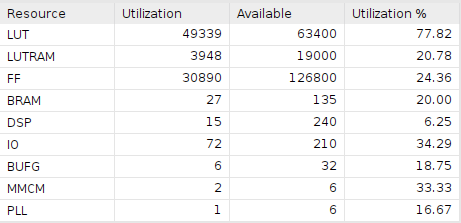
\includegraphics[scale=0.6]{../common/vivado-risk-v Uilization.png}
	\caption{Vivado utilisation report for RISC-V processor}
	\label{fig:LUT_usage}
\end{figure}

Putty was used to connect the to RISC-V processors serial port with a baud rate of 115200. It displayed the Linux boot sequence showing the process was successful (Figure \ref{fig:linux}). Unfortunately, this boot process was extremely slow due to an issue with the udev daemon hindering development with it. There are also issues installing programs with \texttt{apt} in the Linux environment.

\begin{figure}[H]
	\centering
	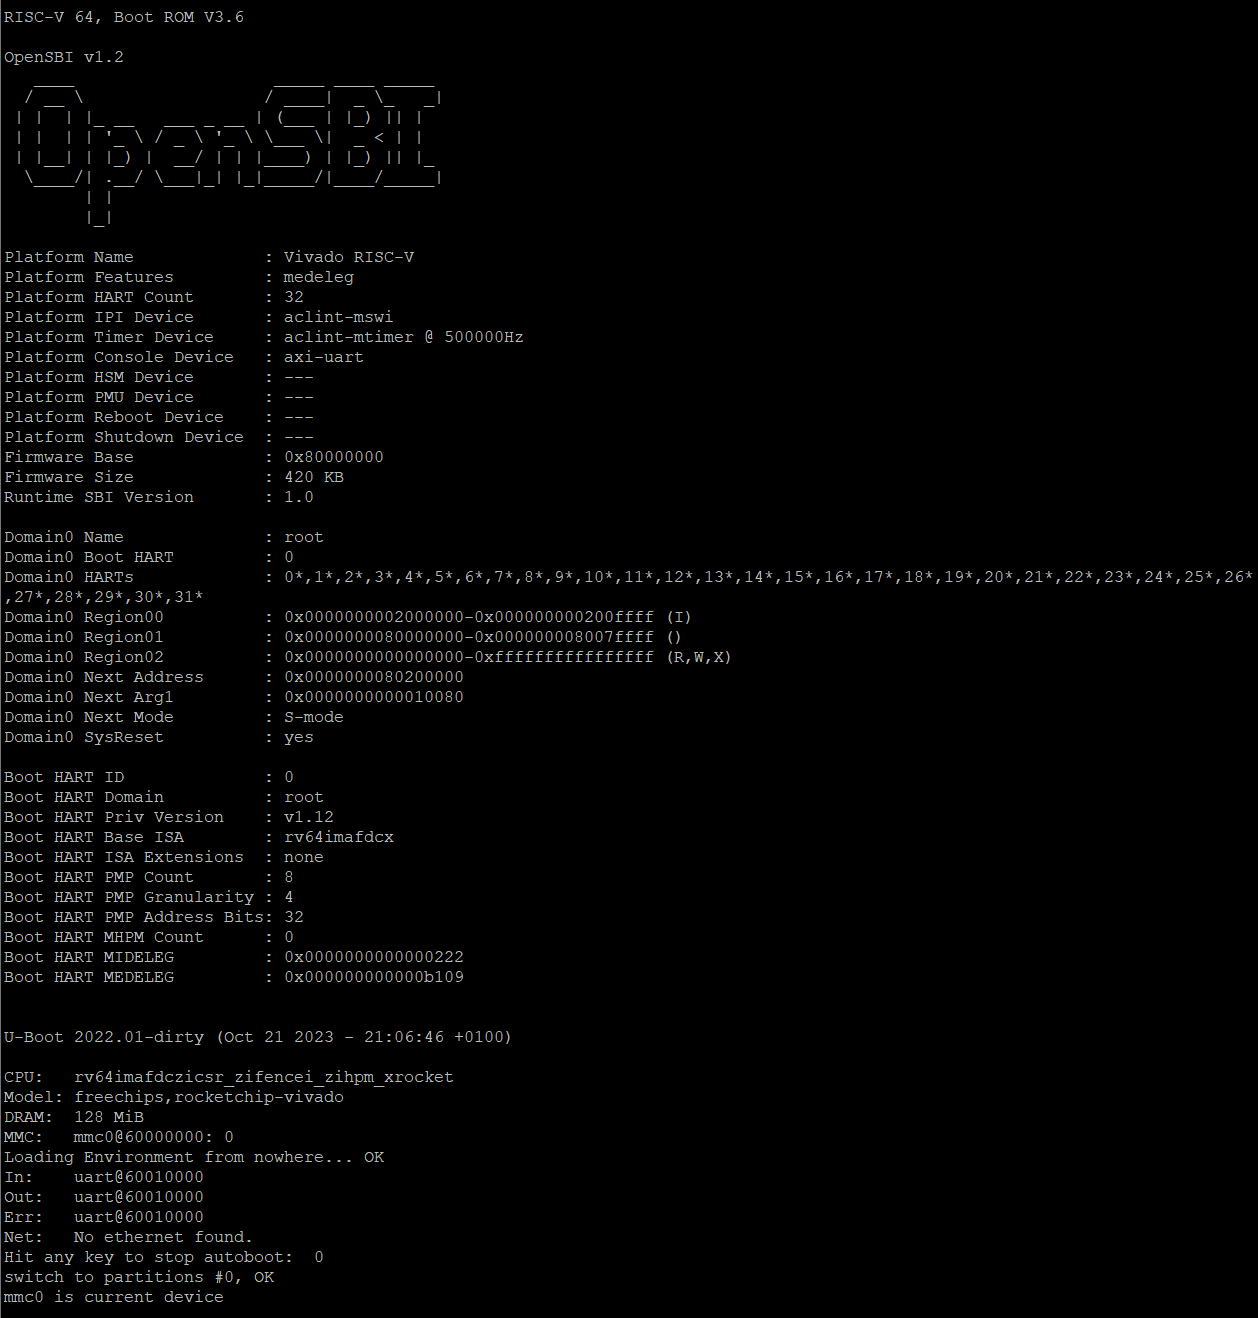
\includegraphics[scale=0.4]{linux.png}
	\caption{Linux booting on the FPGA}
	\label{fig:linux}
\end{figure}

Due to the boot issue with Linux, bare-metal code proved to be a much better solution. The example hello-world bare-metal code from the vivado-risc-v project was successfully run to test the use of bare-metal code (Figure \ref{fig:helloworld}).

\begin{figure}[H]
	\centering
	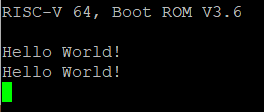
\includegraphics[scale=1]{bare-metal.png}
	\caption{Bare-metal "hello world" script, serial output}
	\label{fig:helloworld}
\end{figure}

\subsection{Adding IP}
The Vivado development environment provides a block view of the project. The AXI interface can be found in the IO block and custom IP blocks can be connected to this to make them available over AXI. To test this pre-made AXI GPIO block \cite{xilinx_gpio} was added and connected to a new master AXI connection on the \texttt{io\_axi\_s} block. The \texttt{axi\_clk} and \texttt{axi\_reset} lines were used for the new IPs clk and reset ports (Figure \ref{fig:gpio_ip}). The output of the GPIO block was connected to the FPGA board LEDs. Under the address editor, a new base address can be assigned to the GPIO block (Figure \ref{fig:address_editor}).

\begin{figure}[H]
	\centering
	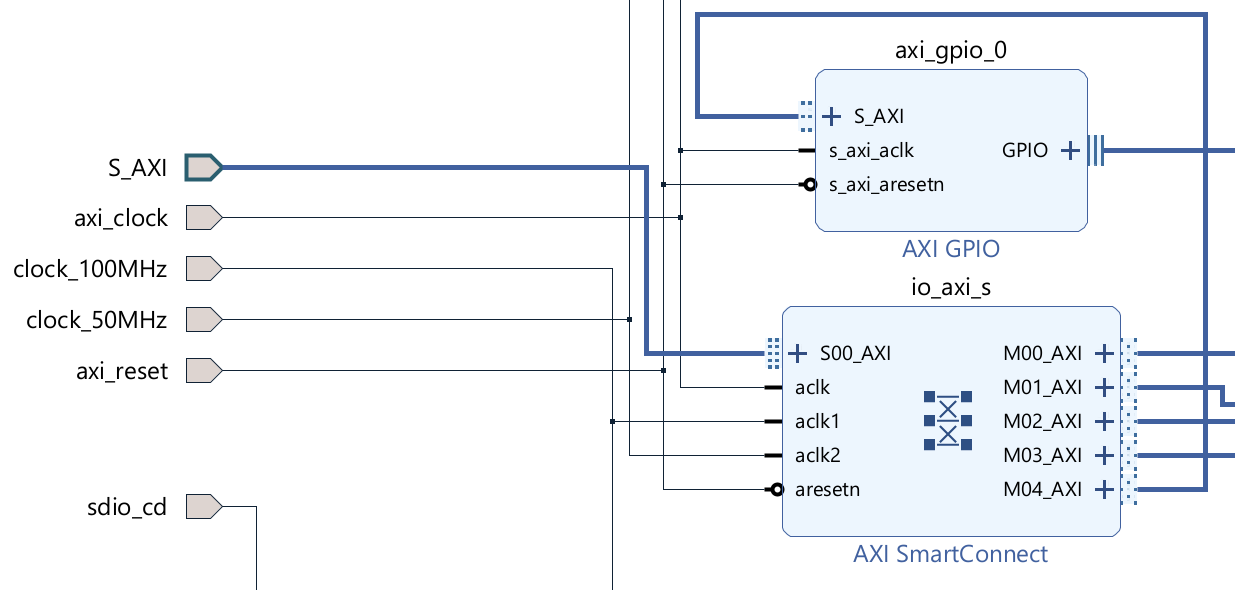
\includegraphics[scale=0.4]{GPIO_IP.png}
	\caption{Vivado IP Block Diagram}
	\label{fig:gpio_ip}
\end{figure}

\begin{figure}[H]
	\centering
	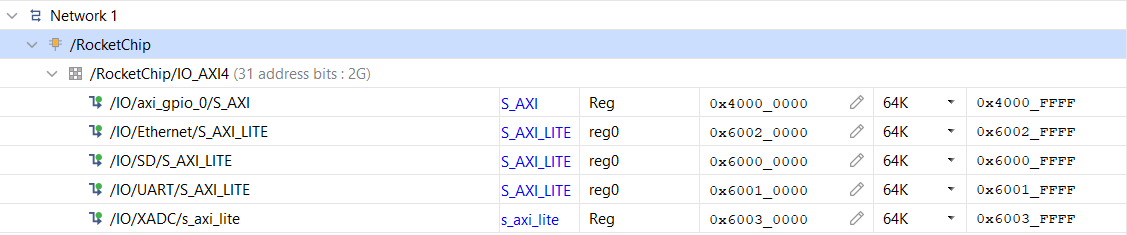
\includegraphics[scale=0.6]{address_editor.png}
	\caption{Vivado Address Editor}
	\label{fig:address_editor}
\end{figure}

Adding this to the device tree in the Linux environment using the example entry was unsuccessful and bare-metal code will be used this was not pursued further. Xilinx provides drivers \cite{xilinx_gpio_driver} for their built-in IP blocks but these are significantly more complicated due to the wide range of devices it must support and include libraries that are not available. The process for interfacing with the IP block is relatively simple. Four 32-bit memory registers start at the assigned base address which represents the data and direction for each of the two 32-bit channels made available. These can be set by writing a uint32 value to a pointer at an address offset from the specified base address. This can be simplified by using a struct (Listing \ref{lst:gpio-struct}).

The example hello-world code was used as a base for developing a script to test this and interact with the serial bus.

\begin{figure}[h]
\begin{lstlisting}[style=CStyle, caption={Definition of a structure to access virtual memory addresses.}, label={lst:gpio-struct}]
typedef struct gpio {
	volatile uint32_t gpio_data;  // Data reg 1
	volatile uint32_t gpio_tri;   // I/O direction reg 1
	volatile uint32_t gpio_data2; // Data reg 2
	volatile uint32_t gpio_tri2;  // I/O direction reg 2
} GPIO;

GPIO * gpio_reg = (GPIO *)base_address;
\end{lstlisting}
\end{figure}

\subsection{Custom AXI IP block}
When creating custom IP blocks in Vivado, a blank block can be generated or a block with a pre-made AXI interface \cite{xilinx_axiip}). To test the use of a custom IP block the pre-made AXI interface was used and custom Verilog code was added to it. This allowed data to be written to one register copied to a second one in hardware and then read back from the new register. A basic shift register was implemented to test processing the data before output but this is not yet working.

\section{Timeline}
The timeline for this project has changed considerably from the specification. It was initially planned to develop the hardware accelerator first and then integrate it into the RISC-V processor. However, it was decided that starting with the processor and building on that was better as the accelerator depends on the system of communication and that depends on the processor. The updated timeline (Table \ref{tab:timeline}) shows this change.

\begin{table}[H]
	\centering
	\resizebox{\textwidth}{!}{
		\begin{tabular}{|c|l|}
			\hline
			\multicolumn{1}{|l|}{Week} & Task                                                               \\ \hline
			2                          & Write specification                                                \\ \hline
			4                          & Generate a working RISC-V processor                                \\ \hline
			6                          & Integrate an IP block into the processors AXI bus                  \\ \hline
			8                          & Integrate a basic custom IP block into the processors AXI bus      \\ \hline
			10                         & Write the progress report                                          \\ \hhline{|=|=|}
			14                         & Develop a custom AXI interface IP block and driver code            \\ \hline
			16                         & Research and design the structure of the hardware accelerator      \\ \hline
			20                         & Implement accelerator in a custom IP block using the AXI interface \\ \hline
			21                         & Design and develop a performance test for the accelerator          \\ \hline
			23/24                      & Write presentation                                                 \\ \hline
			30                         & Write progress report                                              \\ \hline
		\end{tabular}
	}
	\caption{Updated timeline}
	\label{tab:timeline}
\end{table}

The next thing to be developed is a custom AXI interface. This may be based on the code provided by Xilinx or documentation from the developer of ZipCPU \cite{axi_lite_custom}. This will be used to interface with the accelerator by transmitting 32-bit values between the bare-metal code and the hardware. This has been assigned 4 weeks due to it going through the winter holiday.

Next research will be made into methods of building the hardware accelerator and a block design will be made to show how it will be structured before beginning development. Different methods should be considered to find what is best for this project. The designed accelerator can then be implemented in Verilog and connected to the AXI interface block. A bare-metal code driver will pass in the input data and validate the output. This will be used to test the functionality of the accelerator. Input data is currently planned to be stored directly in the code but if time is available it may be modified to allow data to be loaded from the SD card.

A performance test can then be developed and run using hardware and software approaches. This can then be compared to assess the usefulness of the accelerator.

Finally, the presentation and final report can be written.
\section{Project management}
A Trello board (Figure \ref{fig:trello}) has been used to keep track of weekly tasks, resources and issues. The tasks can be marked as "To-Do", "Doing" and "Done". This is reviewed in weekly meetings with the project supervisor and next week's tasks are decided on.

Progress is behind what would be expected if the original timeline had been restructured due to unavoidable personal issues arising and not putting in the hours per week as planned in the specification. A more organised weekly plan will be used to help with time management on the rest of the project and the scope of the project has been changed to allow for the lost time. The switch to using bare-metal code has made the software side considerably simpler and greatly increases the possible speed of development. Using Verilog to develop the hardware instead of Chisle reduces the learning curve allowing for development to start sooner.

\begin{figure}[H]
	\centering
	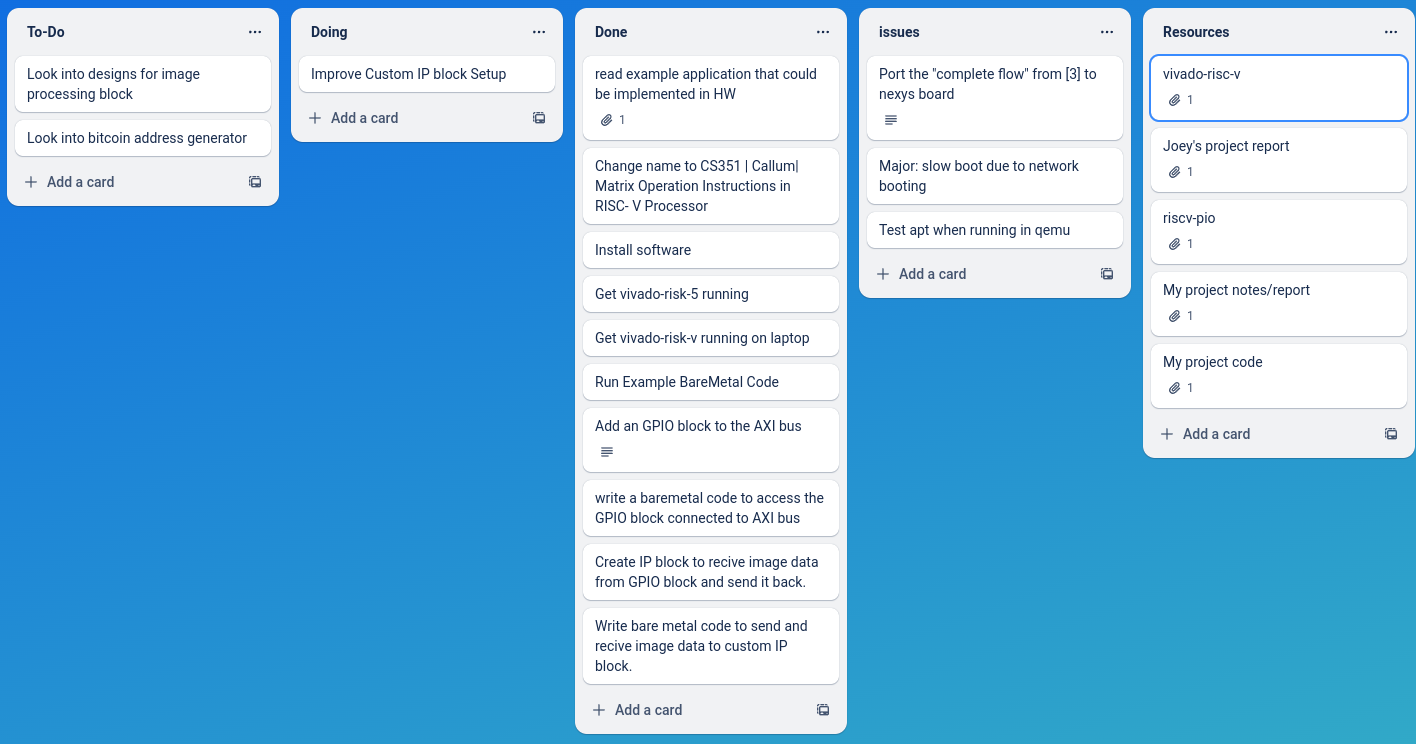
\includegraphics[scale=0.4]{trello}
	\caption{Current status of the project Trello board}
	\label{fig:trello}
\end{figure}

\section{Ethics}
This project does not require working with people and should not present any ethical issues. There should also be no legal issues as there is no intent to profit from this project.

\newpage
\appendix

\section{Project Specification}
\subsection{Introduction}
Many matrix operations involve computing many simpler calculations on the components of the matrix. These calculations are often independent and can be performed in parallel. A processor would compute these sequentially but a specific hardware implementation would be able to compute them in parallel. Adding hardware-based matrix operations to a processor instruction set would allow programs to reduce the number of cycles needed to get the result and so reduce the time taken. As the average clock speed of CPUs has seen very little increase since the early 2000s moving more complicated operations to hardware allows for run time to decrease without decreasing cycle time.

This project aims to develop hardware that can perform matrix operations and integrate that into the instructions of a RISK-V processor to improve the execution time of matrix-heavy programs.

\subsection{Background}
\subsubsection{FPGAs}
As this project will use a hardware implementation, a platform is needed that can allow fast development and iterations on hardware designs. An FPGA (Field Programmable Gate Array) is a semiconductor device based around a matrix of configurable logic blocks \cite{whatisanfpga}. The user can define what logic function these blocks perform and how they are connected using HDL (Hardware Description Language) programming. Hardware can be designed in HDL and constructed on the FPGA without needing to manually build the circuit.

\subsubsection{Matrix Operations}
There are four basic operations with matrices, addition, scalar multiplication, transposition and matrix multiplication. There are multiple algorithms for matrix multiplication. The naive method takes a time of $\mathcal{O}(n^{3})$. More efficient algorithms have been found such as the Refined Laser Method with a time of $\mathcal{O}(n^{2.3728596})$ \cite{alman2020refined}. However, this is a far more complicated algorithm and would only offer better efficiency for large matrices.

In the naive method, each element of the result matrices of these functions can be independently calculated allowing for parallelism. To fully utilise this all elements of the input matrices must be accessible simultaneously which limits the scalability of the input matrix size the design can handle. Block matrix multiplication can be used to split large matrices into smaller blocks that can then be calculated. This allows the hardware to be used to compute larger matrices than it can handle as long as they have a size that is a power of two. Another advantage of the naive method is that a smaller matrix can be computed as a larger matrix by filling in the extra slots with zeros and then removing them from the result.

\subsubsection{RISK-V, Rocket Chip and Chisel}
For this project, a processor is needed to integrate the matrix accelerator with. RISC-V is an open standard instruction set architecture that can be implemented in a variety of devices such as high-performance boards by SiFive and smaller microcontrollers such as Espressif's ESP32-C3. This adoption means that more software is available for the RISC-V instruction such as Debian's risk64 port. To implement a RISC-V core on an FPGA the Rocket Chip Generator will be used. This is an open-source SoC generator that produces synthesizable RTL for implementation on an FPGA. It also allows for the integration of custom accelerators as instruction set extensions \cite{rocketchip} which is needed for this project. The FPGA being used in this project should be able to run one rocket64b core.

Rocket Chip uses the Chisel HDL based on the Scala programming language. This allows for modern programming features to be used and then generate Verilog from this code. The Verilog code can then be synthesised for an FPGA.

\subsection{Literature Review}
The following is a comparison between two papers relevant to this project, Matrix Multiplication Accelerator \cite{matrix_mult_accel} and Implementation of a RISC-V Processor with Hardware Accelerator \cite{risc-v_hard_accel}.

\begin{table}[h]
	\centering
	\resizebox{\textwidth}{!}{%
		\begin{tabular}{c|c|c|}
			\cline{2-3}
			& Matrix Multiplication Accelerator                                                                                                     & \begin{tabular}[c]{@{}c@{}}Implementation of a RISC-V Processor\\ with Hardware Accelerator\end{tabular}                                                       \\ \hline
			\multicolumn{1}{|c|}{Development Board Used}                                                                      & Cyclone V - DE1-SoC with ARM Cortex-A9                                                                                                & \begin{tabular}[c]{@{}c@{}}ZedBoard with Artix-7 FPGA \\ and ARM Cortex-A9 MPCore\end{tabular}                                                                 \\ \hline
			\multicolumn{1}{|c|}{Processor Used}                                                                              & ARM Cortex-A9 HPS                                                                                                                     & \begin{tabular}[c]{@{}c@{}}PULPino (RISC-V) \\ implemented on the FPGA\end{tabular}                                                                            \\ \hline
			\multicolumn{1}{|c|}{\begin{tabular}[c]{@{}c@{}}Connection Used Between\\ Accelerator and Processor\end{tabular}} & Parallel Port on AXI bus                                                                                                              & \begin{tabular}[c]{@{}c@{}}APB bus accessible \\ as virtual memory\end{tabular}                                                                                \\ \hline
			\multicolumn{1}{|c|}{Matrix Algorithm Used}                                                                       & \begin{tabular}[c]{@{}c@{}}Naive method with two approaches, \\ register-based using parallelism \\ and 'single-threaded' memory \\ block approach with pipelining \\ and high clock speeds\end{tabular} & Naive matrix multiplication                                                                                                                                    \\ \hline
			\multicolumn{1}{|c|}{Results}                                                                                     & \begin{tabular}[c]{@{}c@{}}Higher runtime than on HPS \\ but significantly more uniform \\ distribution of results\end{tabular}       & \begin{tabular}[c]{@{}c@{}}Performance improvement by a factor of 4.5 \\ with hardware using just 124 clock cycles \\ compared to 603 in software\end{tabular} \\ \hline
		\end{tabular}%
	}
\end{table}

Implementation of a RISC-V Processor with Hardware Accelerator provided a more in-depth explanation of the project and more useful results. An instruction set extension implementation was not used due to the added complexity so a comparison with the results found in this paper may be useful. Matrix Multiplication Accelerator provided less valuable results as runtime is not as comparable when the hardware and software approaches are running a different clock speeds, 100MHz and 925MHz. It did provide an alternative design for the hardware implementation to improve scalability but block matrix multiplication can allow for the original design to computer larger matrices. 

\subsection{Objectives}
\subsubsection{Hardware-Based Matrix Operations}
\begin{enumerate}
	\item [(Must)]  Design and implement matrix multiplication hardware that can calculate results more efficiently than software. It should work for matrices containing integers and should be able to scale to larger matrices.
	\item [(Could)] Add addition and scalar multiplication functions to the design.
	\item [(Could)] Add support for floating point values to the design.
\end{enumerate}
\subsubsection{Integration to RISC-V Core}
\begin{enumerate}
	\item [(Must)] Generate a RISC-V core and connect it to the matrix accelerator by adding new instructions to the cores instruction set.
	\item [(Must)] Develop software to allow the use of the new instructions in programs.
\end{enumerate}
\subsubsection{Comparison of Hardware Solution Against Software}
\begin{enumerate}
	\item [(Must)] Develop a program that can benchmark the use of matrix operations through software and the hardware accelerator. Run these tests and compare.
	\item [(Could)] Test and compare an implementation that uses software parallelism.
	\item [(Could)] If other matrix functions are implemented compare these to software and see if these extra functions are worth implementing.
\end{enumerate}
			
\subsection{Methodology}
To develop the matrix accelerator a plan-based methodology will be used. The structure of the accelerator will be designed before implementation and then test-driven development will be used when implementing it. It takes a long time to synthesise and generate a bitstream from HDL and can be very hard to debug hardware when it is running on an FPGA. To test more efficiently the HDL it is simulated using the tools built into Vivado for Verilog or with ChiselTest for Chisel code.

To test the performance of the accelerator a benchmark program will be needed. This should test a range of matrix sizes and if able shapes. The test should be run multiple times to find variance in results and should measure runtime and clock cycles.

\subsection{Timeline}
The planned working hours are set out in the table below giving 12 hours a week. This may change depending on what is currently being worked on.

\begin{table}[h]
	\centering
	\begin{tabular}{c|c|c|c|c|c|}
		\cline{2-6}
		& 14:00 & 15:00 & 16:00 & 17:00 & 18:00 \\ \hline
		\multicolumn{1}{|c|}{Monday}    &       &       &       &       &       \\ \hline
		\multicolumn{1}{|c|}{Tuesday}   &       &       & X     & X     & X     \\ \hline
		\multicolumn{1}{|c|}{Wednesday} &       & X     & X     & X     &       \\ \hline
		\multicolumn{1}{|c|}{Thursday}  &       & X     & X     & X     &       \\ \hline
		\multicolumn{1}{|c|}{Friday}    &       &       & X     & X     & X     \\ \hline
	\end{tabular}
\end{table}

The Gantt chart below timetables the progress towards this project. This covers all objectives that must be completed and shows deadline submissions. Additional objectives such as adding extra functionality to the accelerator can be worked if the main objective is completed and there is still allocated time left.

\begin{adjustwidth}{-\oddsidemargin-1in+1cm}{-\rightmargin}
	\centering
	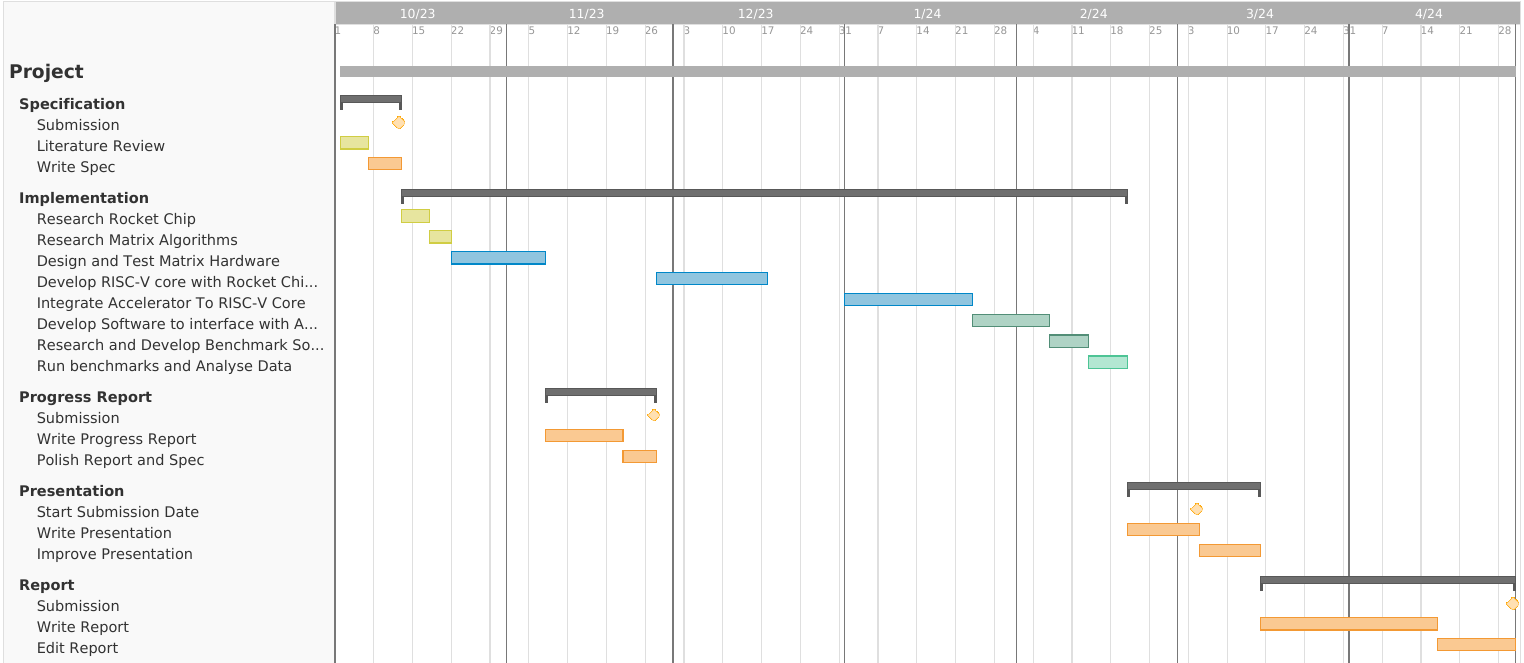
\includegraphics[width=\paperwidth-2cm, frame]{./timeline.png}
\end{adjustwidth}

\subsection{Resources}
This project will require hardware and software resources listed below as well as open-source tools such as Rocket Chip and Git.
\begin{enumerate}
	\item \textbf{FPGA Development Board - Nexys A7-100T} \newline
	This board will be used to synthesise the HDL generated by this project. It is on loan from the School of Engineering.
	\item \textbf{Vivado Design Suit} \newline
	Provides tools to synthesise and analyse HDL for FPGAs. Educational licence through the School of Engineering
	\item \textbf{vivado-risk-v project} \cite{vivado-risk-v} \newline
	An open-source project that generates RISC-V processors for FPGAs using Rocket Chip.
	\item \textbf{Linux Workstation PC} \newline
	A PC capable of running the Vivado Design Suit tools and the Ubunbtu 20.04 environment that is needed for the vivado-risk-v project. My PC fulfils these requirements.
\end{enumerate}

\subsection{Risks}
Three main risks could harm this project. These are listed below along with mitigations and solutions.
\begin{enumerate}
	\item \textbf{Damage to FPGA Development Board} \newline
	This board is on loan from the School of Engineering so a replacement could be obtained. To reduce the chance of damage the board will only be transported when necessary and kept in its protective packaging when not in use.
	\item \textbf{Damage to Workstation} \newline
	Engineering computer labs could be used to run Vivado Design Suit and DCS labs can provide a Linux environment if needed.
	\item \textbf{Data Loss} \newline
	Git version control will be used to track changes and all data relevant to the project will be backed up to GitHub providing an easy way to recover data. A log will be kept of the process to generate data such as the use of vivado-risk-v so it can be repeated if necessary.
\end{enumerate}

\subsection{Legal, Social, Ethical and Professional Issues}
This project should not present any social, ethical or professional issues and does not require working with people. There is no intent to profit from this project so no legal issues should arise. 


\section{Glossary}
\begin{enumerate}
	\item [ FPGA - ] Field-Programmable Gate Array, an integrated circuit designed around configurable logic blocks allowing for custom logic functions to be defined using HDL \cite{whatisanfpga}.
	\item [ HPS - ] Hard Processor System, a physical processor that is not run on an FPGA.
	\item [ LUT - ] Lookup Table, a digital memory element used in FPGAs to implement combinational logic.
	\item [ HDL - ] Hardware Description Language, a language used to describe logic circuits.
	\item [ IC - ] Integrated Circuit, a semiconductor based chip that performs logic on electronic signals.
	\item [ ASIC - ] Application-Specific Integrated Circuit, a custom designed IC for a specific purpose.
	\item [ RISC-V - ] An open standard instruction set for processors \cite{risc}.
	\item [ APB - ] Advanced Peripheral Bus, a low-cost interface for peripheral devices \cite{APB}.
	\item [ AXI - ]  Advanced eXtensible Interface, a protocol used to communicate between the processor and IP blocks \cite{axi}.
	\item [ Bare-metal - ] Software that runs directly on hardware without an operating system.
\end{enumerate}

\bibliographystyle{../common/plainnat}
\bibliography{../common/bibliography}

\end{document}